\chapter{Preliminaries}
%\section{Preliminaries}
In this chapter, we introduce some basic concepts of RDF, Wikidata, SPARQL, and GraphQL. Then, we discuss the differences between SPARQL and GraphQL in terms of ease of use by developers in their applications and expressibility.

%\stepcounter{section}
%\setcounter{secnumdepth}{2}
\section{RDF}
%\subsection{RDF}
The World Wide Web consists of data published in various formats such as PDF, CSV and many forms of plain text \cite{Ruth2013}. Linked Data turns the web into a global database where data can be reused and shared across to everybody. Resource Description Framework (RDF) is a framework used to represent information available in the Web \cite{R.Cyganiak2014}. In the context of graphs, RDF is used for describing and exchanging graphs. The graphs specified by RDF are directed edge-labelled graphs. This means that the edges connect source nodes to target nodes, and have labels. It can be the case that there are multiple edges between the same nodes. However, these edges must have different labels. Figure~\ref{fig:figure 1} shows how knowledge about the chemical element Helium can be represented using a directed edge-labelled graph.

\begin{figure}[h]
  \centering
  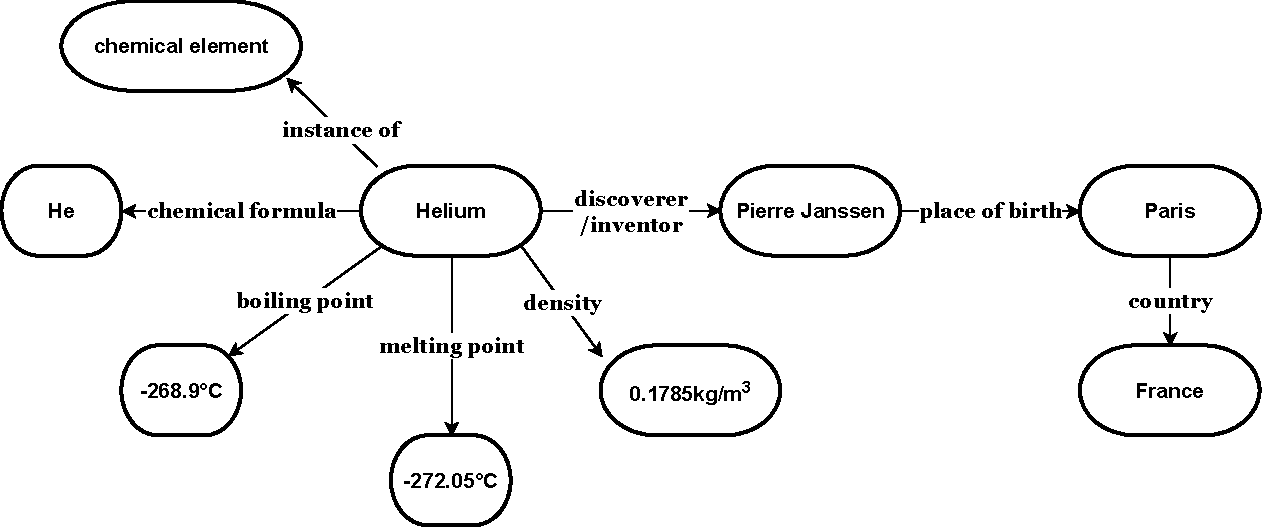
\includegraphics[width=0.80\linewidth]{images/del_graph.drawio.pdf}
  \caption{Directed edge-labelled graph describing Helium}
  \label{fig:figure 1}
\end{figure}

RDF Schema (RDFS) is the Vocabulary Description Language for RDF. Basically, it defines the vocabulary for RDF data. This means that it describes:

\begin{itemize}
	\item the basic concepts and abstract syntax of RDF such as resources and classes\footnote{https://www.w3.org/TR/rdf-concepts/ .}
	\item the formal semantics of RDF\footnote{https://www.w3.org/TR/2014/REC-rdf11-mt-20140225/ .}
	\item the different concrete syntaxes such as Triples, which is shown in section XYZ
\end{itemize}

According to RDFS, resources are divided into groups known as classes. Each member of a class is called an instance of that class, and is itself also a resource. The relationship between subject and object resources is described via RDF properties Essentially, the predicate of an RDF statement is an instance of RDF property. For instance, to identify that a resources is an instance of a class we use the predicate rdf:type which is in turn an instance of RDF property. W3cC provides a thorough documentation on RDF Schema.\footnote{w3.org/TR/2014/REC-rdf-schema-20140225/ .} In Figure 1 we see that Helium is an instance of the class chemical element. The property instance of describes the relation between the subject Helium and object chemical element.
\anas{Is the concept of property and predicate clear?}

In order to exchange graphs across the web we need to identify the resources uniquely. For this we use IRIs which are basically identifiers in RDF. The graph shown in Figure~\ref{fig:figure 1} can be represented using an RDF graph. Formally, the building blocks of RDF graphs are IRIs, literals and blank nodes. These are defined as follows.

\subsection*{IRI}
%\subsubsection{IRIs}
A Uniform Resource Identifier (\acrshort{URI}) is a sequence of a subset of ASCII characters that identifies any web resource by using a name, a location, or both. They have a scheme, authority, path, and query and fragment, where all parts other than scheme and path are optional. URIs are of the form \textbf{scheme:[//authority]path[?query][\#fragment]}. For example, \textit{http://www.wikidata.org/entity/Q560} is an IRI that identifies the chemical element Helium on Wikidata. A Uniform Resource Locator (\acrshort{URL}) is a subset of URI that is used to specify the location of a digital document.

An Internationalized Resource Identifier (\acrshort{IRI}) is a generalized form of URI that helps to distinguish resources with Unicode. Basically, the character set in URI is extended to the Universal Coded Character Set. This enables it to contain any Latin and non-Latin characters except the reserved characters.

In RDF an IRI is used as a name (can be thought of as an ID) for graph nodes. It defines the resources that appears as nodes or edge labels in a RDF graph. There are already several pre-existing IRIs available for common use. New domain specific IRIs can be created based on the application. However, we must ensure there no conflicts with other IRIs available on the web.

\subsection*{RDF Literals}
%\subsubsection{RDF Literals}

An RDF literal consists of three essential elements: a lexical value, a datatype IRI and an optional language tag. The lexical value is a string\footnote{RDF is based on Unicode strings.} that corresponds to a particular literal value in the value space, where value space is the set of all possible values that a datatype can have. There are many datatypes\footnote{A full list is available on the W3C's section on RDF datatypes: www.w3.org/TR/2014/REC-rdf11-concepts-20140225/\#section-Datatypes.} in RDF some of which are string, Boolean, decimal and integer.

The datatype IRI refers to a datatype that defines which strings are valid (belong in the lexical space), the value space and the lexical-to-value mapping \cite{ Bonduel2019}. This mapping is essentially a function that maps each string from the lexical space to an element in the value space. The \acrshort{W3C} standard XML Schema defines the datatypes and their IRIs. For example, decimals are identified by the IRI http://www.w3.org/2001/XMLSchema\#decimal. W3C has a good documentation on the different XML Schema built-in datatypes \cite{ R.Cyganiak2014}.

The optional language tag helps to provide human-readable labels to RDF literals. A literal is a language-tagged string is of the form "string"@language.\footnote{Here language is a well-formed language tag (after \acrshort{BCP47}).} The datatype IRI\footnote{It is never used in syntax.} of such literals is http://www.w3.org/1999/02/22-rdf-syntax-ns\#langString.

RDF literals are used to represent resources that have values belonging to datatypes. Each literal can have only one datatype. For example, the boiling point of Helium would be a RDF literal represented as \texttt{-268.9^^xsd:decimal} and its chemical formula as \texttt{"He"@en}, which is a language-tagged string. Literals are drawn as rectangular nodes in RDF graphs. 

\subsection*{Blank Nodes}
%\subsubsection{Blank Nodes}
A blank node in RDF, also known as a bnode, does not identify a specific resource as IRIs or literals do. It is used as a placeholder for some node, i.e., it is used to say that something with the given relationship exits at the position without specifying what the node is.


\subsection{RDF Graph}
\begin{definition}[RDF Graph]	
An RDF graph is a directed edge-labelled graph composed of a set of triples. A triple, also known as statement, represents the relationship between a subject and an object, linked by a predicate as shown in Figure~\ref{fig:figure 2}. Formally, each triple consist of the following elements:  

\begin{itemize}
	\item a subject node that is an IRI or a blank node
	\item a predicate edge that is an IRI
	\item an object node that is an IRI, a blank node, or a literal
\end{itemize}	
\end{definition}

\begin{figure}[h]
  \centering
  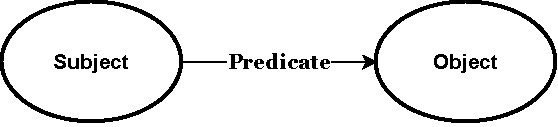
\includegraphics[width=0.75 \linewidth]{images/rdf_relation.drawio.pdf}
  \caption{An RDF graph with Subject and Object nodes connected via a predicate edge}
  \label{fig:figure 2}
\end{figure}



Figure~\ref{fig:figure 3} shows an RDF graph based on our example represented in Figure~\ref{fig:figure 1}. Our main interest is in querying the knowledge graph Wikidata, and so all the data correspond to the resources in its knowledge base. In Wikidata the subject and object represent items, and the predicate represents properties. All items and properties are identified as Unique IDs. For example, the item \textit{Helium} has the ID of \texttt{Q560}, and the property \textit{chemical formula} has the ID \texttt{P274}. These are not understood by humans and have a label property that makes them understood. Moreover, items belong to the namespace \texttt{http://www.wikidata.org/entity/} (prefixed by \texttt{wd}) and properties to \texttt{http://www.wikidata.org/prop/direct/} (prefixed by \texttt{wdt}). As a result, \textit{Helium} would have the IRI \texttt{http://www.wikidata.org/entity/Q560} (\texttt{wd:Q560}) and \textit{chemical formula} the IRI \texttt{http://www.wikidata.org/prop/direct/P274} (\texttt{wdt:P274}). Section XYZ gives an elaborate understanding of entities and the namespaces they belong to in Wikidata.

From Figure~\ref{fig:figure 3} we understand that \textit{Helium} \texttt{(\gls{Q560})} is an \textit{instance of} \texttt{(P31)} of \textit{chemical element} \texttt{(Q11344)}. It has a human understandable english \textit{label} called \textit{helium} and the \textit{chemical formula} \texttt{(P274)} of \textit{He}. Its \textit{boiling point} \texttt{(P2102)}, \textit{melting point} \texttt{(P2102)} and \textit{density} \texttt{(P2054)} are \textit{-268.9~°C}, \textit{0.1785~°C} and \textit{-272-05~kg/m3} respectively. Helium has a \textit{discoverer/inventor} \texttt{(P61)} by the name of \textit{Pierre Janssen} \texttt{(Q298581)}. His \textit{place of birth} \texttt{(P19)} was \textit{Paris} \texttt{(Q90)} that belongs to the \textit{country} \texttt{(P17)} of \textit{France} \texttt{(Q142)}.

\begin{figure}[h]
  \centering
  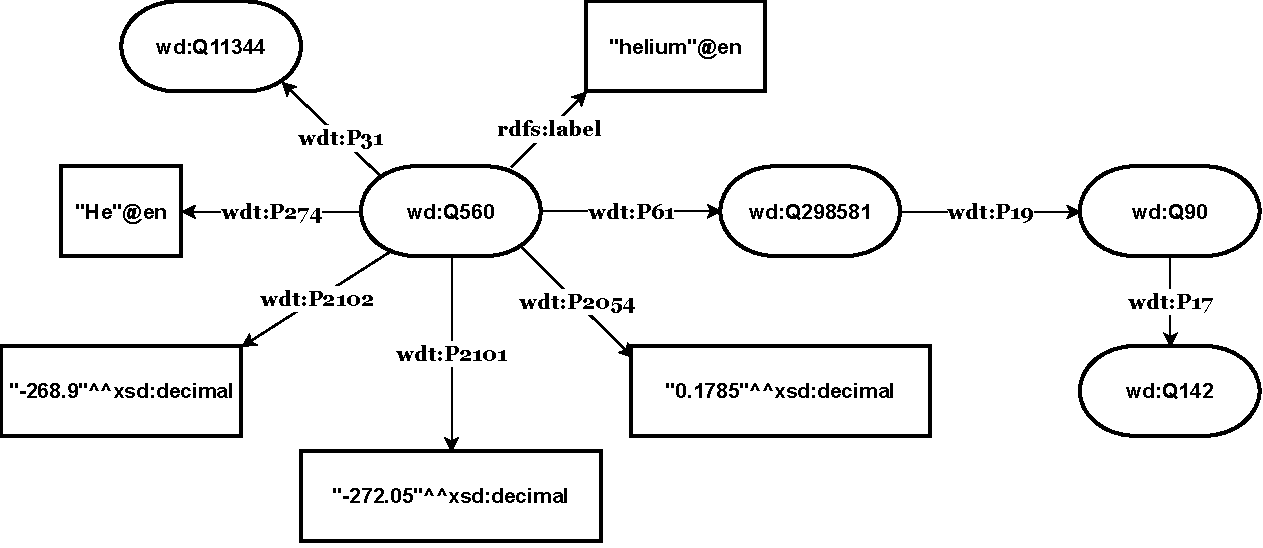
\includegraphics[width=0.75 \linewidth]{images/rdf_graph.drawio.pdf}
  \caption{RDF graph describing Helium}
  \label{fig:figure 3}
\end{figure}

%\begin{table}[b!]
%	\begin{center}
%		\caption{Abbreviation/IDs and their meanings.}
%		\label{tab: table 1}
%		\begin{tabular}{c|c}
%%			\textbf{Benchmarking tool} & \textbf{Resource monitoring tool} & \textbf{License} & \textbf{Updated} \\ \hline
%			wd & http://www.wikidata.org/entity/ \\ \hline
%			wdt & http://www.wikidata.org/prop/direct/ \\ \hline
%			rdfs & http://www.w3.org/2000/01/rdf-schema\# \\ \hline
%			Q560 & Helium \\ \hline
%			Q298581	& discoverer/inventor \\ \hline
%			Q90 & Paris \\ \hline
%			P31	& instance of \\ \hline
%			P274 & chemical formula \\ \hline
%			P2102 & boiling point \\ \hline
%			P2101 & melting point \\ \hline
%			P2054 & density \\ \hline
%			P61	& discoverer/inventor \\ \hline
%			P19	 & place of birth \\ \hline
%			P625 & coordinate location
%		\end{tabular}
%	\end{center}
%\end{table}


\subsection{Serialisations}
For exchanging graphs across the web, we need a syntactical representation of RDF. There are different formats available, the most common ones are N-Triples, Turtle, JSON-LD, RDF/XML and RDFa. In this report we focus on N-Triples and Turtle.

\subsubsection{N-Triples}
N-Triples represents RDF graphs in a simple line-based format.\footnote{Full specification available at: https://www.w3.org/TR/n-triples/ .} Every triple is encoded in a single line. The IRIs are written within pointy brackets and literals are written as lexical value\textasciicircum \textasciicircum datatype-IRI. Blank nodes are represented as \_:stringID, where stringID can be any string used to identify the blank node in the document. After every element of a triple there is a whitespace, and all the lines end with a dot. We can use comments using hash symbol after the end of every triple in a line or in a single dedicated line, and they are treated as white spaces. The files are saved with a \textit{.nt} extension.

Listing~\ref{listing:listing1} shows the representation of the RDF graph in Figure~\ref{fig:figure 3} in N-triples format. We have given line breaks for better readability.

\begin{minipage}{\linewidth}
\begin{lstlisting}[columns=fullflexible, label=listing:listing1, caption={RDF graph represented in N-triples syntax}, language=SPARQL]

<http://www.wikidata.org/entity/Q560> <http://www.wikidata.org/prop/direct/P31> 
%\phantom{<http://www.wikidata.org/entity/Q560> <http://www.}%<http://www.wikidata.org/entity/Q11344> .
		                                                
<http://www.wikidata.org/entity/Q560> <http://www.w3.org/2000/01/rdf-schema#label> 
%\phantom{<http://www.wikidata.org/entity/Q560> <http://www.}%"helium"@en .

<http://www.wikidata.org/entity/Q560> <http://www.wikidata.org/prop/direct/P274> 
%\phantom{<http://www.wikidata.org/entity/Q560> <http://www.}%"He"@en .

<http://www.wikidata.org/entity/Q560>  <http://www.wikidata.org/prop/direct/P2102> 
%\phantom{<http://www.wikidata.org/entity/Q560> <http://www.}%"-268.9"^^<http://www.w3.org/2001/XMLSchema#decimal> .

<http://www.wikidata.org/entity/Q560> <http://www.wikidata.org/prop/direct/P2101> 
%\phantom{<http://www.wikidata.org/entity/Q560> <http://www.}%"0.1785"^^<http://www.w3.org/2001/XMLSchema#decimal> .

<http://www.wikidata.org/entity/Q560> <http://www.wikidata.org/prop/direct/P2054> 
%\phantom{<http://www.wikidata.org/entity/Q560> <http://www.}%"-272.05"^^<http://www.w3.org/2001/XMLSchema#decimal> .

<http://www.wikidata.org/entity/Q560> <http://www.wikidata.org/prop/direct/P61> 
%\phantom{<http://www.wikidata.org/entity/Q560> <http://www.}%<http://www.wikidata.org/entity/Q298581> .

<http://www.wikidata.org/entity/Q298581> <http://www.wikidata.org/prop/direct/P19> 
%\phantom{<http://www.wikidata.org/entity/Q560> <http://www.}%<http://www.wikidata.org/entity/Q90> .

<http://www.wikidata.org/entity/Q90> <http://www.wikidata.org/prop/direct/P17> 
%\phantom{<http://www.wikidata.org/entity/Q560> <http://www.}%<http://www.wikidata.org/entity/Q142> . 

\end{lstlisting}
\end{minipage}

\subsubsection{Turtle}
Turtle is an easy to read representation of RDF graphs. It extends the N-Triples format by providing several simplifications.\footnote{Full specification available at: https://www.w3.org/TR/turtle/ .} We can use prefix declarations and base namespaces at the beginning of the file to shorten IRIs. Turtle allows us to avoid repetition. We can use a semicolon at the end of a line instead of a dot if we know the next line has the same subject. Consequently, the next line will only have a predicate and object omitting the subject. Also, we can use a comma at the end of a line if we know the next line will start with the same subject and predicate. Analogously, the next line will only have a an object omitting the subject and the predicate. Blank nodes are represented using only square brackets. Additionally, we can provide predicate-object pairs within the square brackets to give further triples keeping the blank node as the subject. Turtle also provides a shorthand syntax for writing numbers. Numbers of the datatype integer, decimal and double can be written without quotes and datatype-IRIs. Boolean values can be written directly as either "\textit{true}" or "\textit{false}". The files are saved with a \textit{.ttl} extension.

Listing~\ref{listing:listing2} shows the representation of the RDF graph in Figure~\ref{fig:figure 3} in Turtle format. 

\begin{minipage}{\linewidth}
\begin{lstlisting}[label=listing:listing2, caption={RDF graph represented in Turtle syntax}, language=SPARQL]

PREFIX wd: <http://www.wikidata.org/entity/>
PREFIX wdt: <http://www.wikidata.org/prop/direct/>
PREFIX rdfs: <http://www.w3.org/2000/01/rdf-schema#>
PREFIX xsd: <http://www.w3.org/2001/XMLSchema#>
PREFIX geo: <http://www.opengis.net/ont/geosparql#>

wd:Q560 wdt:P31 wd:Q11344 ;
%\phantom{wd:Q560 }% rdfs:label "helium"@en ;
%\phantom{wd:Q560 }% wdt:P274 "He"@en ;
%\phantom{wd:Q560 }% wdt:P2102 -268.9 ;
%\phantom{wd:Q560 }% wdt:P2101 0.1785 ;
%\phantom{wd:Q560 }% wdt:P2054 -272.05 ;
%\phantom{wd:Q560 }% wdt:P61 wd:Q298581 .
wd:Q298581 wdt:P19 wd:Q90 .
wd:Q90 wdt:P17 wd:Q142 .

\end{lstlisting}
\end{minipage}


\section{Wikidata}
%\subsection{Wikidata}
Wikidata is a free and publicly available knowledge base that can be read and edited by both humans and machines. It is one of the many projects by Wikimedia Foundations such as Wikipedia, Wikibooks, Wikimedia Commons and Wikitionary.  Wikidata was created in 2012 at Wikimedia Deutschland by a community of volunteers. These volunteers edit and control all content. As of December 2022, Wikidata has more 23000 active editors.\footnote{https://wikidata.wikiscan.org/ .} Wikidata provides a website where data can be viewed and also edited \cite{Foundationa}.

One of the original purposed behind the creation of Wikidata was to help its sister projects. Initially, Wikipedia and its sister projects used to maintain their own lists of interlanguage links. This refers to links between Wikipedia articles about the same topic but in different languages. After 2012, these interlanguage links were provisioned via Wikidata. Wikidata is also used to display data shown inside the pages in Wikipedia. The usage of this mainly depends on the language of the Wiki. For instance, in the case of some languages, parts of the Wikipedia pages are created automatically from the data in Wikidata. Others, especially those of smaller languages that are not widely used, use Wikidata to create placeholder pages when an article may not be in their respective language. In 2018, around 59\% of Wikidata information was used in English Wikipedia articles, although mostly for external identifiers and coordinate locations \cite{Wikipedia2017}. 

Wikidata stores information in the form of structured data in a database \cite{Tharani2021}. This is not the case for its sister projects as they contain unstructured data stored. The information on their web pages is not directly given a structure in the form of tables or lists. Wikidata acts as a central storage for these projects and focuses on providing a structure for their data \cite{Wikidata2014}. Additionally, Wikidata also supports linked data. This means that the data stored can be linked to datasets and databases like Google Books and OmegaWiki. Wikidata can also be used for quality checks against Wikipedia articles. This is useful when information about a specific topic needs to be known and the solution is easily found by querying the knowledge graph, in this case Wikidata.

Moreover, there is also a wide range of commercial and research oriented applications for Wikidata. This is due to the fact that it has a large amount of real world data. For instance, Wikidata has external usages in many large organizations such as Eurowings, Google, Apple and Amazon. This includes tasks such as data integration, authority control, identity providing and data-driven journalism. In the field of research, Wikidata is used for collecting test data for knowledge graph related algorithms and training data for machine learning projects.

Wikidata is built on the RDF framework. However, it does not define its resources in terms of RDF. Instead, it has its own model known as Wikibase data model.\footnote{https://www.mediawiki.org/wiki/Wikibase/DataModel.} This distinction creates an abstract layer between its model and RDF. Consequently, there are similarities with RDF’s W3C standards but there are also some important differences. For instance, the Wikidata property \textit{instance of} (\texttt{P31}) is semantically equivalent to the property \textit{rdf:type} in RDF. The value of \texttt{P31} is a class that is itself an item. Wikidata offers an explanation for some of the standards properties in Wikidata that correspond to the ones in RDF \cite{Foundation}. Statements (triples) in Wikidata can have annotations (qualifiers) and references.

The basic elements in Wikidata are entities, also known as resources. These are mainly items and properties. The next section describes entities in Wikidata. 

\subsection{Entities}
Wikidata maintains its data structure by pages. Each entity has a dedicated page for itself. Basically, every element on which Wikidata has structured data is known as an entity\cite{Erxleben2014}. Entities are identified by an unique ID and not by names or labels. Currently, Wikidata has mainly three types of entities – item, property and lexeme. Other extensions can define new entity types such as MediaInfo and subentities like Form and Sense. We will discuss about items and properties. The rest are out of the scope of this report.

Items are real-world objects, concepts or events. According to RDF terminology, items are instances and classes. Instead of a human understandable name, they are identified by a QID - an ID prefixed with the letter "Q" and followed a number. Items in Wikidata belong to the main namespace - \textit{http://www.wikidata.org/wiki/QID}. Every item constitutes of the following main parts - labels, descriptions, aliases, sitelinks and statements\cite{Erxleben2014}.

Labels, descriptions and aliases are multilingual which help to find the respective item. Since items are identified by an ID, these are used to identify the items clearly. Sitelinks provide links about an individual item in Wikidata to external pages on other Wikimedia sites such as Wikipedia and its other sister projects. The most important part are statements. 

A statement in Wikidata consists of a claim, references and a rank. Claims are property-value pairs, which along with the item form a RDF triple, where the item is the subject. Claims can also contain optional qualifiers that provide some additional information for the claim. This information is a property-value pair that refers to the main part of the statement instead of the item itself\cite{Erxleben2014}. References point to resources that support the claim. An item can have several statements for the same property, and all of them might not necessarily be important or relevant. Ranks are used as a quality factor to distinguish between several statements. A Wikidata statement can have one of three types of ranks - "normal", "preferred" and "deprecated". By default, a statement has the normal rank unless changed to preferred or deprecated. A statement with preferred rank means it should be given priority over the normal ranked statements. A deprecated rank indicates that the statement is incorrect or under discussion, and it may have a reference. Deprecated statements are kept either for the sake for completion or to prevent users from constantly adding or removing them. Wikidata has around 100 million items\footnote{https://grafana.wikimedia.org/d/000000167/wikidata-datamodel.} and around 1.43 billion item statements as of December 2022.\footnote{https://grafana.wikimedia.org/d/000000175/wikidata-datamodel-statements.}

Figure~\ref{fig:figure 4} shows an excerpt of the Wikidata page on the item Helium.\footnote{https://www.wikidata.org/wiki/Q560.} We can see Helium has the QID of Q560, and has labels, descriptions and aliases in different languages. It has a sitelink for the item in Wikipedia offered in 186 languages. Helium has a statement that indicates that Helium has the instance of property with chemical element as the values. The property-value pairs follows, hydrogen and followed by, lithium are qualifiers. This statement hence gives us the information that Helium is an instance of chemical element, and it comes after the element hydrogen and if followed by the element lithium. This statement has no references and has the normal rank (indicated by the middle portion greyed).

\begin{figure}[h]
  \centering
  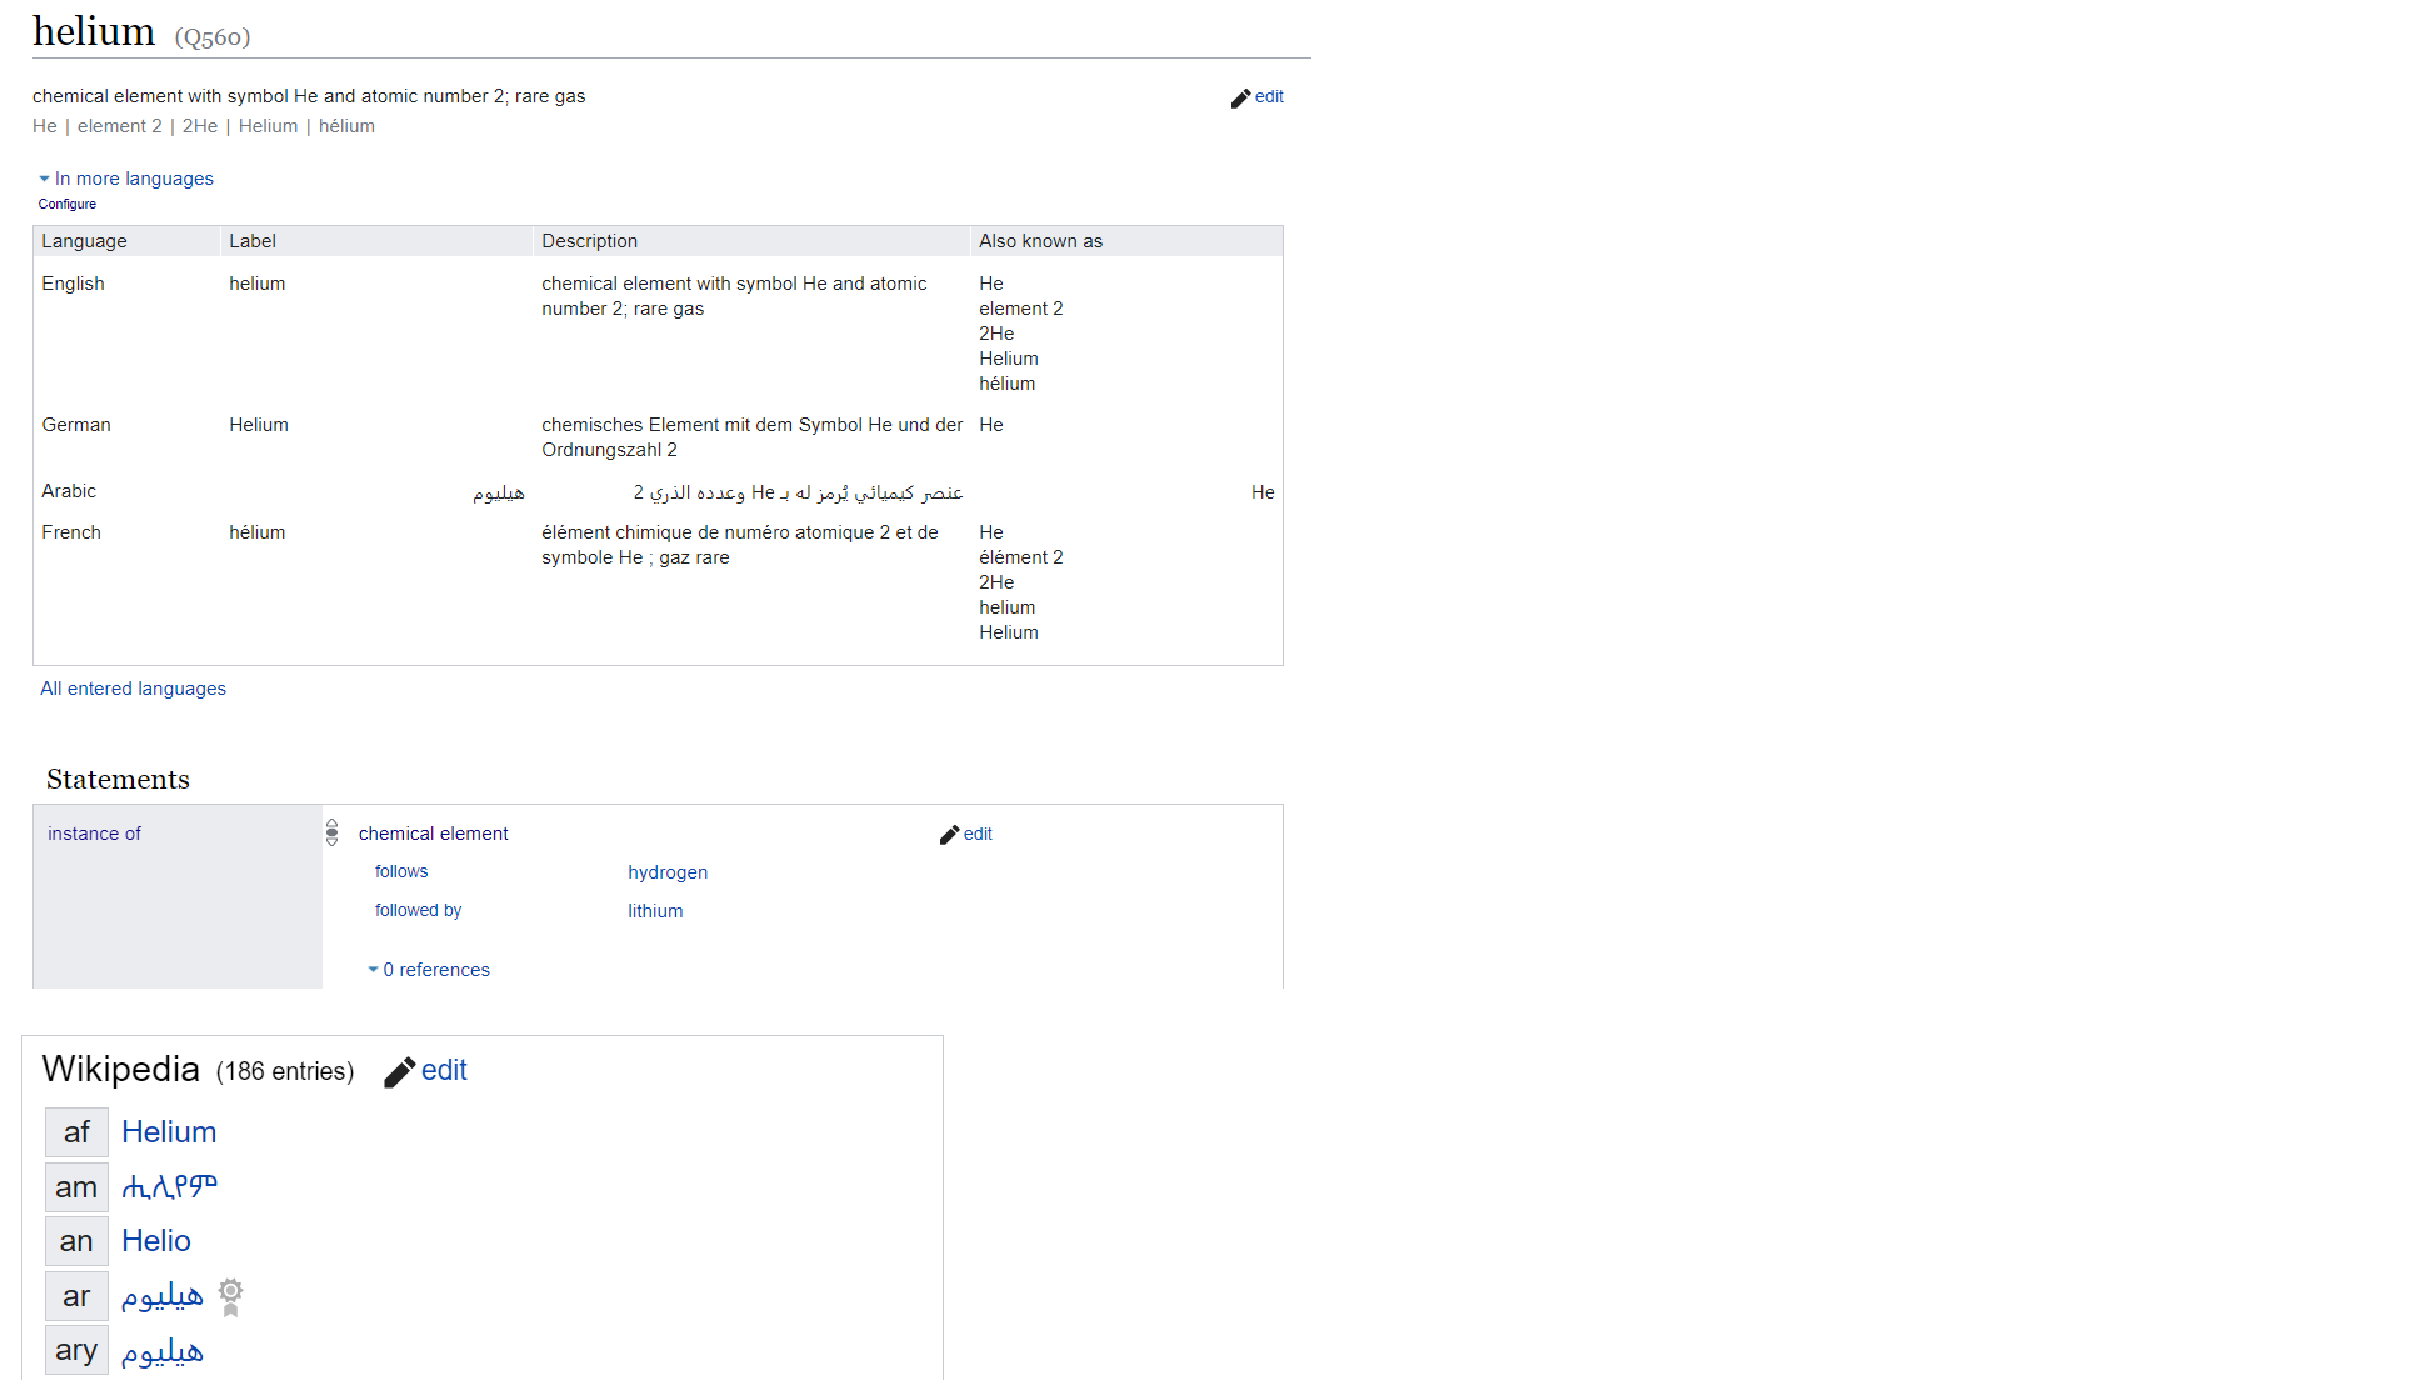
\includegraphics[width=0.75 \linewidth]{images/helium.pdf}
  \caption{An excerpt of the page on \textit{Helium} in Wikidata}
  \label{fig:figure 4}
\end{figure}

Properties in Wikidata resemble RDF properties and are essentially attributes for describing entities. They are identified by a PID - an ID prefixed with the letter "P" and followed a number. They belong to the property namespace in wikidata - http://www.wikidata.org/wiki/Property:PID. Like items, they also have labels, descriptions, aliases and statements but no sitelinks. However, they has an additional part called datatype that determines which values they accept, such as string, quantity and time.\footnote{Wikidata provides a list of all the datatypes: https://www.wikidata.org/wiki/Special:ListDatatypes.}

Figure~\ref{fig:figure 5} shows an excerpt of the property instance of page on Wikidata.\footnote{https://www.wikidata.org/wiki/P31.} The property has a PID of P31 along and with multilingual labels, descriptions and aliases. From the statement we understand that it this property also has an instance of property with Wikidata property being the value. The statement has no qualifiers or references, and has the normal rank. The instance of property accepts the datatype item as a value.

\begin{figure}[h]
  \centering
  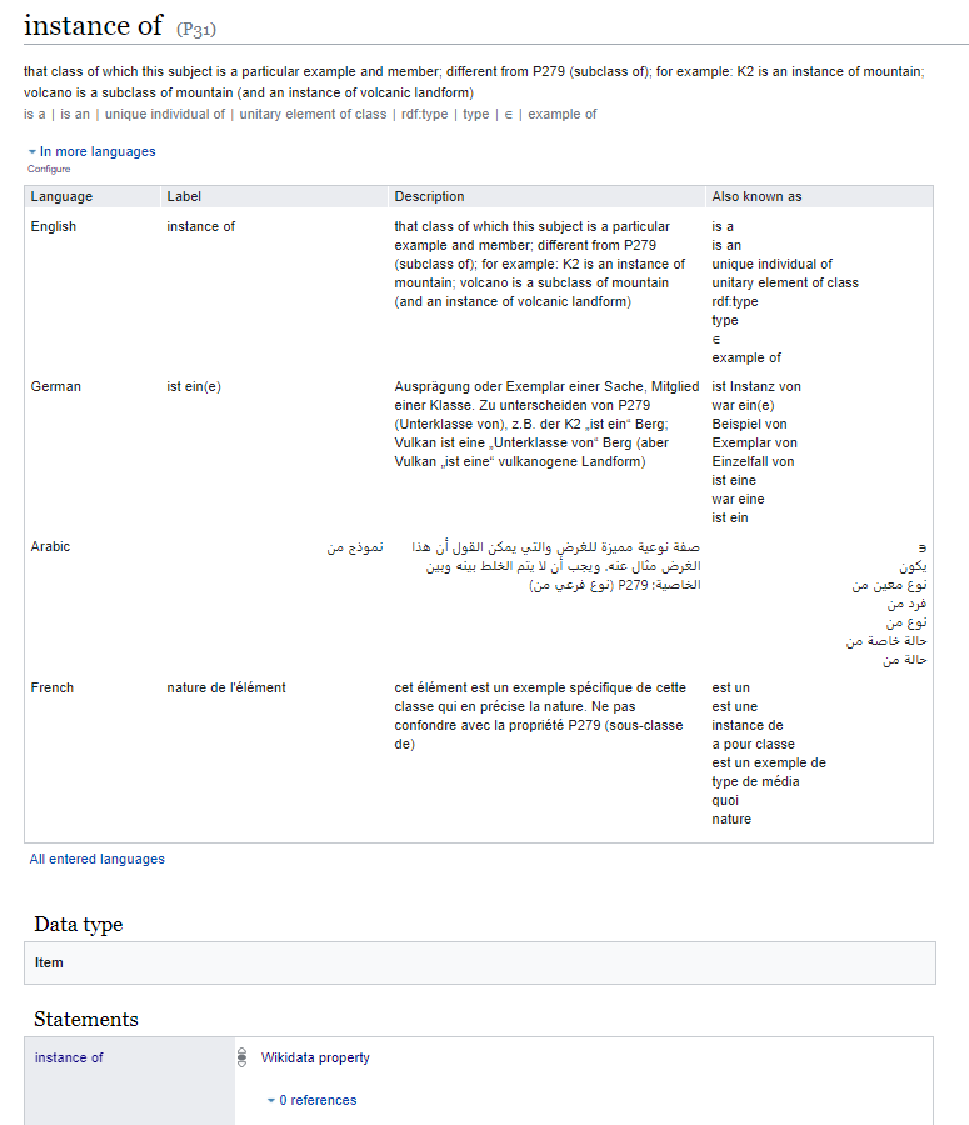
\includegraphics[width=0.75 \linewidth]{images/instance_of.pdf}
  \caption{An excerpt of the page on \textit{instance of} in Wikidata}
  \label{fig:figure 5}
\end{figure}

\subsection{Querying Wikidata}

The easiest and most popular way to query Wikidata is through the Wikidata Query Service (WDQS). This is Wikidata's SPARQL endpoint. We can use this service two ways. Firstly, we can write queries in SPARQL directly on the web user interface of the service\footnote{https://query.wikidata.org/ .} and obtain the results in different formats like table, tree, graph, etc. Secondly, the service can also be used progmatically by submitting GET or POST requests.\footnote{https://query.wikidata.org/sparql.}

Another popular way to query Wikidata is by using the Wikidata API.\footnote{https://www.wikidata.org/wiki/Special:ApiSandbox.} However, this API should mainly be used when we want to edit the contents of Wikidata or get data about entities like revision history.

Wikidata dumps is useful when we know our result set will be significantly large or if we want to set up our own local query service. These dumps are full exports of all the available entities in Wikidata.\footnote{https://dumps.wikimedia.org/ .} To get started you should download the latest complete dump.\footnote{https://dumps.wikimedia.org/wikidatawiki/latest/ .} Wikidata also mentions some other ways to accessing Wikidata's data like Search and Linked Data Fragments endpoint, the complete list and usage of which can be found on Wikidata's Data Access webpage \cite{ Wikidata2022}.


\section{SPARQL}
%\subsection{SPARQL}
SPARQL Protocol and RDF Query Language (SPARQL)\footnote{https://www.w3.org/TR/sparql11-overview/ .} is a W3C recommended query language for RDF. This means it allows to query any data source that can be mapped to RDF. It is also a HTTP-based protocol for linked open data on the web. This enables the transmission of SPARQL queries and results between a client and a SPARQL engine. The first working draft for SPARQL was released in 2004 and it became a W3C Recommendation in 2008 \cite{Perez2009}. 

Queries in SPARQL are based on matching graph patterns and can be used to retrieve, add or delete data in the RDF based dataset. In section XYZ we saw that RDF data is based on triples - subject, object and predicate. Consequently, a query in SPARQL consists of a set of triple patterns. Each of the elements of the triple can be a variable (a string beginning with ? or \$) that needs to be queried. The solution to the variables is obtained by matching the query patterns to the triples in the dataset.

There are four forms of queries - SELECT, ASK, CONSTRUCT and DESCRIBE. 
\begin{itemize}
\item SELECT queries select some or all the pattern matches and provides the results in a tabular format
\item ASK queries check whether there is at least one match and the result is true or false
\item CONSTRUCT queries create an RDF graph based on the query results
\item DESCRIBE queries return a RDF graph providing additional information on each results
\end{itemize}

In our work, we only consider SELECT queries. These consist of the following major blocks:
\begin{itemize}
\item Prologue: PREFIX and BASE keywords that function similarly to those in RDF turtle format
\item Select clause: SELECT keyword followed by either a list of variables and variable assignments, or by *
\item Where clause: WHERE keyword followed by a query graph pattern to be matched
\item Solution set modifiers: Change the set of solutions using modifiers such as LIMIT and OFFSET
\end{itemize}

The select and where clauses are mandatory, the rest being optional. Other optional features are filters, groups, query operators such as UNION, OPTIONAL and BIND, and aggregates. A full specification for the query language can be found on the official W3C documentation\cite{Seaborn}.

Listing~\ref{listing:listing3} shows an example of querying Wikidata using SPARQL. We want to get a a list of all chemical elements, along with their English labels, that have a chemical formula, boiling point, melting point, density, an inventor/discoverer, birth place of that inventor/discoverer and the country that the place belongs to. Since there might be several results, we are limiting them to five using the LIMIT keyword. The namespace http://www.wikidata.org/entity/ is used for items when querying. We are interested in the truthy values of the properties and so the namespace http://www.wikidata.org/prop/direct/ is used for properties. Truthy values are essentially the values for which the statement has the best non-deprecated rank. This means that if a statement has preferred rank then that statement is considered to be truthy. Otherwise, the normal ranked statement is taken to be truthy. The PREFIX is optional since Wikidata recognizes the short forms wd and wdt automatically. Turtle syntax that we saw in section XYZ can be applied in SPARQL. The query can be run in Wikidata's query service.\footnote{https://query.wikidata.org/ .}  

\begin{minipage}{\linewidth}
\begin{lstlisting}[label=listing:listing3, caption={Querying Wikidata with SPARQL}, language=SPARQL]

PREFIX wd: <http://www.wikidata.org/entity/>
PREFIX wdt: <http://www.wikidata.org/prop/direct/>
SELECT *
WHERE {
  ?element wdt:P31 wd:Q11344 ;
  %\phantom{?element }% wdt:P274 ?element_formula ; 
  %\phantom{?element }% wdt:P2102 ?boiling_point ;
  %\phantom{?element }% wdt:P2101 ?melting_point ;
  %\phantom{?element }% wdt:P2054 ?density ;
  %\phantom{?element }% wdt:P61 ?discoverer .
  ?discoverer wdt:P19 ?place_birth .
  ?place_birth wdt:P17 ?country .
  FILTER(LANG(?element_label)="en")
}LIMIT 5

\end{lstlisting}
\end{minipage}

Table 1 shows the results obtained in a tabular form. Among the results, there is the element Helium (Q560) that we have used as an example in Fig 1 and Fig 3. 

\begin{table}[h]
	\begin{center}
		\caption{Results of the SPARQL query in Listing 2}
		\label{tab: table 1}
		\begin{tabular}{ccccccccc}
		
%		\textbf{element} & \textbf{element_formula} & \textbf{element_label} & \textbf{boiling_point} & \textbf{melting_point} & \textbf{density} & \textbf{discoverer} & \textbf{place_birth} & \textbf{country} \\ \hline
			\toprule
			
			\textbf{element} & \textbf{element\textunderscore formula} & \textbf{element\textunderscore label} & \textbf{boiling\textunderscore point} & \textbf{melting\textunderscore point} & \textbf{density} & \textbf{discoverer} & \textbf{place\textunderscore birth} & \textbf{country} \\ 
		
			\midrule
			
			wd:Q560 & He & helium	& -268.9 & -272.05 & 0.1785 & wd:Q298581 & wd:Q90 & wd:Q142 \\
			
			wd:Q560 & He & helium & -268.9 & -272.05 & 0.1785 & wd:Q950726 & wd:Q4093 & wd:Q145 \\ 
			
			wd:Q560 & He & helium & -268.9 & -272.05 & 0.1785	 & wd:Q127959 & wd:Q623765 & wd:Q145 \\ 
			
			wd:Q670 & Si & silicon & 4271 & 2570	& 2.329	& wd:Q151911 & wd:Q1451001 & wd:Q34 \\ 
			
			wd:Q568	& Li & lithium	& 1317	& 180.5	& 0.535	& wd:Q313568 & wd:Q10495519 & wd:Q34 \\
			
			\bottomrule

		\end{tabular}
	\end{center}
\end{table}

\section{GraphQL}

GraphQL (Graph Query Language) is an open source query language for APIs (Application Programming Interfaces) and a runtime for executing those queries against existing data. It describes data structured in a graph format – a collection of objects (nodes) connected to each other by some kind of relationships (edges). Runtime is usually implemented by a server.

GraphQL is usually served over HTTP through a GraphQL server. A GraphQl server consists of two main parts – schema and resolver. The API developers create a schema that is strictly typed and describes all the possible data a client can query using the service. The schema specifies object types and fields along with operations on those types. The object type represents the kind of object that can be requested by a client. 

There are three operations types – query, mutation and subscription.  We look at the query operation in this chapter; the other two are outside the scope of this report. Queries are used to fetch or read data. When compared to REST (Representational State Transfer),  queries operations in GraphQL are similar to GET requests. A resolver in GraphQL server is a function that is associated with every field and contains instructions on how to process that particular field. In other words, the resolver is responsible for retrieving a value from the data source. 

GraphQL is data agnostic, i.e., it is not concerned where the data source is located. The data could be stored in any source such as a database or a micro-service as shown in Figure XYZ. With a single API call, GraphQL can aggregate data from multiple sources and resolve the data to the client. This is one of the advantages GraphQL has over REST API where the latter would require several HTTP calls to access data from multiple sources. Apart from being data agnostic, GraphQL is also language agnostic. This means that GraphQL services, such as the schema and resolvers, can be written in any programming language such as JavaScript or Python. 

For the sake of human readability, GraphQL specification has its own Schema Definition Language (SDL). It is simple to write and understand schemas in SDL, and is similar to the language that we use to write queries. Listing XYZ shows a schema written in SDL. This schema can be in the GraphQL server against which clients can send queries for instances of chemical elements that have a name, chemical formula and boiling point. The exclamation mark means that the corresponding field is non-nullable and it is expected that GraphQL will give a value when the field is queried. A complete guide on schemas and types can be found on the official documentation from GraphQL.\footnote{https://graphql.org/learn/schema/ .} 

\begin{minipage}{\linewidth}
\begin{lstlisting}{gql.py:GraphqlLexer -x}[label=listing:listing4, caption={Schema used to query a chemical element}]
type Query{
	chemicalElement: ChemicalElement
}

type ChemicalElement{
	name: String!
	chemicalFormula: String!
	boilingPoint: Float!
}

\end{lstlisting}
\end{minipage}

Listing XYZ shows a query that can be used against this schema and the results that could be obtained. The results obtained are in JSON format. The official GraphQL website provides a comprehensive documentation on querying a GraphQL server. \footnote{ https://graphql.org/learn/queries/ .} 

\begin{minipage}{\linewidth}
\begin{lstlisting}[label=listing:listing5, caption={Query to fetch chemical elements and their properties}]
query QueryChemicalElement (limit 2){
    chemicalElement{
		name
		chemicalFormula
		boilingPoint
	}
}
\end{lstlisting}
\end{minipage}

\begin{minipage}{\linewidth}
\begin{lstlisting}[label=listing:listing5, caption={Query to fetch chemical elements and their properties}]
{
	"data":{
		"chemicalElement":{
			"name": "helium",
			"chemicalFormula": "He",
			"boilingPoint": -268.9
		},
		{	
			"name": "silicon",
			"chemicalFormula": "Si",
			"boilingPoint": 4271
		}
	}
}

\end{lstlisting}
\end{minipage}

\section{GraphQL vs SPARQL}

GraphQL and SPARQL are query languages developed with different goals in mind. GraphQL was designed mainly to wrap REST APIs in a graph like shape. This would allow fetching related data in a single request with the aid of schemas. In REST API, the same would require calling multiple endpoints. SPARQL, on the other hand, was developed mainly as a query language for RDF graphs.

SPARQL is immensely popular in the field of research and academia. However, it has not seen much growth in commercial applications. GraphQL, on the other hand, is more popular among software and web developers. There are some valid reasons for this.  

Firstly, many developers are still not familiar with the Linked Data model of RDF and SPARQL. They are more used to working with technologies such as GraphQL and RESTAPIs. Secondly, GraphQL is simple to learn and work with since it has human-oriented syntax. Among other things, this benefits application development. SPARQL however, proves to be more complex. It has more syntactic verbosity owing to the descriptive nature of writing queries. The produced output from SPARQL queries contains a lot of unnecessary metadata that is not useful for web developers and need to be further parsed for using in web applications \cite{Lisena2018}. 

Moreover, retrieval of data from knowledge graphs using SPARQL is time consuming and proves to be a steep learning curve, the reason being that there is limited documentation available for proper ontology descriptions and examples of using queries for SPARQL endpoints \cite{Angele2022}. One of the other reasons for using GraphQL over SPARQL is that developers are more equipped in using nested objects that GraphQL offers \cite{Taelman2018}. They lack the experience to work with triples which is the main foundation of SPARQL. Moreover, fewer supporting tools like libraries and frameworks exist for working and developing with SPARQL than with GraphQL \cite{Taelman2018}. 

On the other hand, SPARQL also has some advantages over GraphQL. SPARQL queries represent full graphs while those of GraphQL represent trees \cite{Taelman2018}. This make SPARQL more expressive. RDF provides a system to build detailed structures from the meaning of data, and is hence more complete and capable than GraphQL schemas \cite{Dresslar2019}. Since SPARQL works with the schema organization of RDF, this makes it more powerful than GraphQL. With SPARQL we can write complex queries that can be used to retrieve or modify data \cite{Angele2022}. As a result it is capable to satisfy many complex use cases.

Also since GraphQL alone has no notion of semantics \cite{Taelman2018}, a schema needs to be defined by the GraphQL API developers for every interface they want the client to query. This makes it difficult to integrate data returned when querying multiple different sources. SPARQL however supports federated queries which makes it more powerful and rich. Lastly, when using GraphQL we cannot uniquely identify resources on the web but which is possible using URIs with SPARQL. In other words, GraphQL has no notion of global identifiers \cite{Taelman2018}.

\textcolor{red}{Talk also about differences in terms of complexity and expressivity}
